\section{Problem Formulation}\label{sec:formulation}

\subsection{Geometry and kinematics}\label{sec:geometry}
We consider a spherical core--shell particle of outer radius $b$ whose concentric, impermeable core has radius
$a=\gamma b$, $0\le\gamma\le1$ (\cref{fig:schematic}). The limit $\gamma=0$ is a homogeneous porous sphere and
$\gamma=1$ an impermeable sphere. The particle is immersed in an incompressible Newtonian fluid of density $\rho$ and
viscosity $\mu$ that fills the half-space $z>0$ (domain 1, outside $r=b$). The half-space $z<0$ (domain 3) is a
homogeneous, isotropic, rigid and stationary porous medium of permeability $k_p$ and Brinkman (effective) viscosity
$\mu_p$, saturated with the same fluid; it models a glycocalyx or mucus layer whose thickness exceeds the range of the
disturbance. The shell $a<r<b$ (domain 2) is a porous medium of permeability $k_s$ and Brinkman viscosity $\mu_s$.
The particle centre is at $\bx_0=h\be_z$ with $h>b$, and we write $r=|\bx-\bx_0|$, with $(r,\theta,\varphi)$ spherical
coordinates centred at $\bx_0$. The dimensionless gap is
\begin{equation}
  \varepsilon=\frac{h-b}{b}.\label{eq:gap}
\end{equation}
The particle translates without rotating at the velocity
\begin{equation}
  \bU(t)=\operatorname{Re}\!\left[U\be\,e^{-i\omega t}\right],\qquad
  \be=\be_z\ \text{(normal oscillation)}\quad\text{or}\quad\be=\be_x\ \text{(parallel oscillation)},
  \label{eq:kinematics}
\end{equation}
with angular frequency $\omega$ and complex amplitude $U$. All fields are written as
$\bu(\bx,t)=\operatorname{Re}[\bu(\bx)e^{-i\omega t}]$ and $p(\bx,t)=\operatorname{Re}[p(\bx)e^{-i\omega t}]$; we use the
same symbol for a field and its complex amplitude.

\begin{figure}[t]
  \centering
  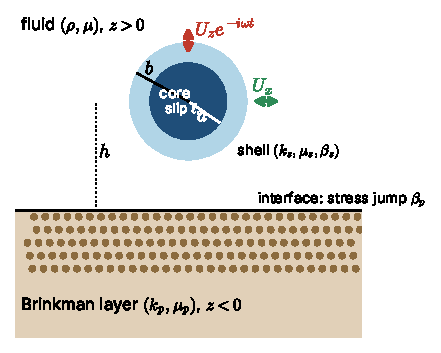
\includegraphics[width=0.8\linewidth]{figures/fig1_schematic.pdf}
  \caption{Core--shell particle (impermeable core of radius $a$ with Navier slip $\ell_c$; Brinkman shell of
  permeability $k_s$, viscosity $\mu_s$ and surface stress-jump coefficient $\beta_s$) oscillating with velocity
  $U\be\,e^{-i\omega t}$, normal ($\be_z$) or parallel ($\be_x$), at centre height $h$ above a semi-infinite Brinkman
  layer of permeability $k_p$ and viscosity $\mu_p$, coupled to the clear fluid through a stress-jump condition with
  coefficient $\beta_p$.}
  \label{fig:schematic}
\end{figure}

\subsection{Modelling assumptions}\label{sec:assumptions}
\begin{assumption}[Small amplitude]\label{as:linear}
The displacement amplitude $|U|/\omega$ is small compared with $b$ and with the gap $h-b$. Convective inertia
$\rho(\bu\cdot\nabla)\bu$ is then negligible relative to the unsteady inertia $\rho\,\partial_t\bu$, and all boundary
conditions are imposed at the mean particle position. The problem is linear and time-harmonic.
\end{assumption}
\begin{assumption}[Rigid porous matrices]\label{as:rigid}
The solid matrices of the shell and the layer are rigid: the shell matrix moves with the particle and the layer matrix
is at rest. Elastic deformation, which is the subject of
Ref.~\onlinecite{batalha2026elasto}, is not considered. ``Soft'' refers to hydrodynamic permeability, as in
soft-particle electrokinetics.
\end{assumption}
\begin{assumption}[Brinkman description]\label{as:brinkman}
Flow in each porous region obeys the unsteady Brinkman equation with Darcy drag relative to the local matrix. The
interfacial momentum transfer at both fluid--porous interfaces follows the Ochoa-Tapia--Whitaker (OTW) stress
jump~\cite{ochoatapia1995momentum}. The Beavers--Joseph slip model~\cite{beavers1967boundary} is recovered from the same
equations as the limit of a Darcy-dominated porous side (\cref{rem:bj}).
\end{assumption}
\begin{assumption}[Prescribed translation]\label{as:norotation}
The particle is driven in pure translation (an AFM colloidal probe glued to a cantilever, or a particle in an imposed
acoustic field), so no torque-free rotation is allowed. Translation--rotation coupling near a wall enters the force at
higher order in $b/h$ than is retained in \cref{sec:closure}.
\end{assumption}
\begin{assumption}[Thick layer]\label{as:thick}
The porous layer is modelled as a half-space. This is appropriate when its thickness exceeds both the Brinkman
screening length $\sqrt{k_p\mu_p/\mu}$ and the distance $h$, so that the reflected disturbance does not feel the
underlying substrate.
\end{assumption}

\subsection{Governing equations}\label{sec:equations}
In the clear fluid (domain 1) the unsteady Stokes equations hold:
\begin{equation}
  -i\omega\rho\,\bu^{(1)}=-\nabla p^{(1)}+\mu\nabla^2\bu^{(1)},\qquad\nabla\cdot\bu^{(1)}=0 .
  \label{eq:stokes}
\end{equation}
In the shell (domain 2) the Darcy drag acts on the velocity relative to the moving matrix:
\begin{equation}
  -i\omega\rho\,\bu^{(2)}=-\nabla p^{(2)}+\mu_s\nabla^2\bu^{(2)}-\frac{\mu}{k_s}\left(\bu^{(2)}-U\be\right),
  \qquad\nabla\cdot\bu^{(2)}=0 .
  \label{eq:shell}
\end{equation}
In the porous layer (domain 3),
\begin{equation}
  -i\omega\rho\,\bu^{(3)}=-\nabla p^{(3)}+\mu_p\nabla^2\bu^{(3)}-\frac{\mu}{k_p}\bu^{(3)},
  \qquad\nabla\cdot\bu^{(3)}=0 .
  \label{eq:layer}
\end{equation}
Taking the curl of \cref{eq:stokes,eq:shell,eq:layer} shows that the vorticity in each domain obeys a modified Helmholtz
equation $(\nabla^2-\lambda_j^2)\,\curl\bu^{(j)}=\bm 0$ with the complex screening parameters
\begin{equation}
  \lambda_f^2=-\frac{i\omega\rho}{\mu},\qquad
  \lambda_s^2=\frac{\mu/k_s-i\omega\rho}{\mu_s},\qquad
  \lambda_p^2=\frac{\mu/k_p-i\omega\rho}{\mu_p},
  \qquad\operatorname{Re}\lambda_j>0 .
  \label{eq:lambdas}
\end{equation}
The real part of $1/\lambda_f$ is the viscous penetration depth $\delta_v=\sqrt{2\mu/\rho\omega}$. Inside the porous
media the vortical disturbance is screened by both the Darcy drag and the unsteady inertia; whichever dominates sets
the decay length.

The stress tensor in domain $j$ is $\bsig^{(j)}=-p^{(j)}\bI+\mu_j(\nabla\bu^{(j)}+\nabla\bu^{(j)\mathsf T})$ with
$\mu_1=\mu$, $\mu_2=\mu_s$, $\mu_3=\mu_p$.

\subsection{Boundary and interface conditions}\label{sec:bcs}
Let $\bn$ be the outward unit normal of the relevant sphere and $\bm\Pi=\bI-\bn\bn$ the tangential projector.

\emph{Core surface} $r=a$ (impermeability and Navier slip of length $\ell_c$):
\begin{equation}
  \left(\bu^{(2)}-U\be\right)\cdot\bn=0,\qquad
  \bm\Pi\cdot\left(\bu^{(2)}-U\be\right)=\frac{\ell_c}{\mu_s}\,\bm\Pi\cdot\bsig^{(2)}\cdot\bn .
  \label{eq:bc_core}
\end{equation}

\emph{Shell surface} $r=b$ (continuity of velocity and normal stress; OTW stress jump with coefficient $\beta_s$):
\begin{subequations}\label{eq:bc_shell}
\begin{align}
  \bu^{(1)}&=\bu^{(2)},\qquad \bn\cdot\bsig^{(1)}\cdot\bn=\bn\cdot\bsig^{(2)}\cdot\bn,\\
  \bm\Pi\cdot\left(\bsig^{(2)}-\bsig^{(1)}\right)\cdot\bn&=\frac{\beta_s\mu}{\sqrt{k_s}}\,
  \bm\Pi\cdot\left(\bu^{(1)}-U\be\right).
\end{align}
\end{subequations}
For an impermeable particle ($\gamma=1$) the shell is absent and \cref{eq:bc_shell} is replaced by
$\bu^{(1)}\cdot\bn=U\be\cdot\bn$ and $\bm\Pi\cdot(\bu^{(1)}-U\be)=(\ell_c/\mu)\,\bm\Pi\cdot\bsig^{(1)}\cdot\bn$ on $r=b$,
which is the slip sphere of Ref.~\onlinecite{faltas2021axisymmetric}.

\emph{Layer surface} $z=0$ (continuity of velocity and normal stress; OTW stress jump with coefficient $\beta_p$):
\begin{subequations}\label{eq:bc_plane}
\begin{align}
  \bu^{(1)}&=\bu^{(3)},\qquad \sigma^{(1)}_{zz}=\sigma^{(3)}_{zz},\\
  \sigma^{(3)}_{\tau z}-\sigma^{(1)}_{\tau z}&=\frac{\beta_p\mu}{\sqrt{k_p}}\,u^{(1)}_\tau,\qquad\tau\in\{x,y\}.
\end{align}
\end{subequations}

\emph{Far field:} $\bu^{(1)}\to\bm 0$ as $|\bx|\to\infty$ in $z>0$, and $\bu^{(3)}\to\bm 0$ as $z\to-\infty$.

\begin{remark}[Limits of the layer]\label{rem:bj}
As $k_p\to0$ ($\alpha_p\to\infty$) the layer velocity vanishes and \cref{eq:bc_plane} reduces to no slip on a rigid
impermeable wall, the configuration of Zhang \emph{et al.}~\cite{zhang2023unsteady}. For $\mu_p=\mu$, $\beta_p=0$ and
$k_p\to\infty$ the layer becomes indistinguishable from the fluid and the interface disappears. For a Darcy-dominated
layer ($\alpha_p\gg\Wo$), the layer velocity varies over the Brinkman length $\sqrt{k_p\mu_p/\mu}$. Eliminating the
porous side then yields an effective slip condition for the clear fluid of Beavers--Joseph
type~\cite{beavers1967boundary}, whose slip coefficient depends on $\beta_p$ and $\mu_p/\mu$. In this sense the present
formulation contains the Beavers--Joseph interface as a special case. \TODO{authors: decide whether to add the explicit
reduction, cf.\ Ref.~\onlinecite{elsayed2026effect}}
\end{remark}

\subsection{Dimensionless formulation}\label{sec:nondim}
Lengths are scaled by $b$, velocities by $U$, pressures and stresses by $\mu U/b$, and forces by $\mu bU$. The problem
then depends on the groups in \cref{tab:groups}. In particular,
\begin{equation}
  \lambda_f b=e^{-i\pi/4}\Wo,\qquad
  (\lambda_s b)^2=\frac{\alpha_s^2-i\Wo^2}{\mu_s/\mu},\qquad
  (\lambda_p b)^2=\frac{\alpha_p^2-i\Wo^2}{\mu_p/\mu}.
  \label{eq:lambdas_nd}
\end{equation}
\Cref{eq:lambdas_nd} shows the key competition: inertia overtakes the Darcy drag in the layer when $\Wo\gtrsim\alpha_p$,
and in the shell when $\Wo\gtrsim\alpha_s$.

\begin{table}[t]
\caption{Dimensionless groups and bio-relevant ranges.}
\label{tab:groups}
\begin{ruledtabular}
\begin{tabular}{lll}
Group & Definition & Range \\
\hline
Womersley number & $\Wo=b\sqrt{\rho\omega/\mu}$ & $10^{-2}$ (AFM) -- $10^{1}$ (acoustofluidics)\\
Gap & $\varepsilon=(h-b)/b$ & $1$ -- $5$ (this work)\\
Core ratio & $\gamma=a/b$ & $0$ -- $1$ ($0.5$--$0.95$ for cells, liposomes)\\
Shell permeability & $\alpha_s=b/\sqrt{k_s}$ & $1$ -- $50$\\
Layer permeability & $\alpha_p=b/\sqrt{k_p}$ & $3$ -- $300$ (glycocalyx, mucus)\\
Stress-jump coefficients & $\beta_s,\ \beta_p$ & $-1$ -- $1$\\
Core slip length & $\hat\ell_c=\ell_c/b$ & $0$ -- $0.5$\\
Viscosity ratios & $\mu_s/\mu,\ \mu_p/\mu$ & $1$ (this work)\\
\end{tabular}
\end{ruledtabular}
\end{table}

\subsection{Hydrodynamic force and observables}\label{sec:observables}
By symmetry the force on the particle is parallel to $\be$:
\begin{equation}
  \bF=\oint_{r=b}\bsig^{(1)}\cdot\bn\,\dd S=F\be,\qquad F=F_\infty+F_{\rm int},
  \label{eq:force}
\end{equation}
where $F_\infty$ is the force in an unbounded fluid and $F_{\rm int}$ is the interaction force induced by the layer. We
decompose the interaction force into a dissipative part and a reactive (inertial) part:
\begin{equation}
  F_{\rm int}=-\gamma_{\rm int}\,U-m_{\rm int}\,\frac{\dd U}{\dd t}
  =\left(-\gamma_{\rm int}+i\omega m_{\rm int}\right)U,
  \label{eq:decomposition}
\end{equation}
so that $\gamma_{\rm int}$ is the wall-induced damping coefficient and $m_{\rm int}$ the wall-induced added mass. In
dimensionless form,
\begin{equation}
  \hat\gamma_{\rm int}=\frac{\gamma_{\rm int}}{6\pi\mu b}=-\frac{\operatorname{Re}\hat F_{\rm int}}{6\pi},\qquad
  \hat\chi_{\rm int}=\frac{\omega m_{\rm int}}{6\pi\mu b}=\frac{\operatorname{Im}\hat F_{\rm int}}{6\pi},\qquad
  \frac{m_{\rm int}}{m_f}=\frac{9}{2}\,\frac{\hat\chi_{\rm int}}{\Wo^2},
  \label{eq:observables}
\end{equation}
with $\hat F=F/(\mu bU)$ and $m_f=\tfrac43\pi\rho b^3$ the displaced fluid mass. The phase of the total resistance is
$\phi=\arg(-F/U)$.

\begin{remark}[Sign convention]\label{rem:sign}
In \cref{eq:decomposition} a positive $m_{\rm int}$ increases the effective inertia. For a probe of effective mass $M^*$
on a spring (an AFM cantilever), the resonance frequency then shifts by
$\Delta\omega_0/\omega_0\simeq-m_{\rm int}/(2M^*)$ when the shift is small. A crossover of $m_{\rm int}$ from
negative to positive values as $\Wo$ increases is therefore the crossover of the frequency shift from positive to
negative reported in Ref.~\onlinecite{zhang2023unsteady}.
\end{remark}

\begin{definition}[Crossover Womersley numbers]\label{def:woc}
At fixed geometry and material parameters, the crossover Womersley numbers are the roots of $m_{\rm int}(\Wo)=0$. We
call a root \emph{upward} ($\Wo_c^{\uparrow}$) when $m_{\rm int}$ changes from negative to positive with increasing
$\Wo$, and \emph{downward} ($\Wo_c^{\downarrow}$) otherwise. For a rigid sphere near a rigid wall there is a single
upward root, denoted $\Wo_c$.
\end{definition}

\subsection{Objective and difficulty}\label{sec:objective}
The problem is to find, for each $(\Wo,\varepsilon,\gamma,\alpha_s,\beta_s,\hat\ell_c,\alpha_p,\beta_p)$ and both
directions $\be$, the complex interaction force $F_{\rm int}$ and from it $\gamma_{\rm int}$, $m_{\rm int}$, $\phi$ and
the crossover set $\{\Wo_c^{\uparrow},\Wo_c^{\downarrow}\}$. Three features make this hard:
\begin{enumerate}
\item The boundaries have different symmetries: spherical surfaces at $r=a,b$ and a plane at $z=0$. No single
      coordinate system separates the problem, and bispherical coordinates do not apply to Brinkman layers with a stress
      jump.
\item Each domain has its own complex screening length (\cref{eq:lambdas}). The fluid disturbance contains both a
      long-range potential part (decaying as $r^{-3}$) and a vortical part confined to a layer of thickness
      $|\lambda_f|^{-1}$; the porous interface converts each part into the other.
\item The parameters of interest span the transition between viscous ($\Wo\ll1$) and inertial ($\Wo\gg1$) regimes,
      and between Darcy-dominated ($\alpha_p\gg\Wo$) and inertia-dominated ($\alpha_p\ll\Wo$) layers. Any asymptotic
      expansion in one of these parameters fails somewhere in the region of interest.
\end{enumerate}
\Cref{sec:analysis} therefore treats the sphere exactly in spherical harmonics and the plane exactly in Fourier space,
and couples them through the $l=1$ moments of the field that alone determine the force.
